\documentclass[11pt]{article}

\usepackage{graphicx} % for including graphics
\usepackage{amsmath} % useful maths macros, including \text
\usepackage{listings}
\usepackage{gensymb}
\usepackage{textcomp}
\usepackage{afterpage}
\usepackage{apacite}
\usepackage{acronym}
\usepackage{caption}
\usepackage{subcaption}

\usepackage{tikz}
\usetikzlibrary{shapes.geometric,arrows}
\tikzstyle{startstop} = [rectangle, rounded corners, text width=3cm,minimum width=3cm,
minimum height=1cm, text centered, draw=black, fill=red!30]
\tikzstyle{io} = [trapezium, trapezium left angle=70,trapezium right angle=110, minimum width=3cm, minimum height=1cm, text centered, draw=black, fill=blue!30]
\tikzstyle{process} = [rectangle, minimum width=3cm, text width=3cm,minimum height=1cm, text centered draw=black, fill=orange!30]
\tikzstyle{decision} = [diamond, minimum width=3cm, text width=3cm,minimum height=1cm, text centered, draw=black, fill=green!30]
\tikzstyle{arrow} = [thick,->,>=stealth]


\usepackage[bibstyle=ieee,citestyle=numeric-comp]{biblatex} % the cite style lets multiple refs in one bracket
\addbibresource{shared_resources/master.bib}
\renewcommand*{\multicitedelim}{\addcomma} % stops spaces between refs in single square bracket
% \usepackage{multicol}
% \usepackage{float}
\usepackage[a4paper, total={6in, 7.5in}]{geometry} % set the paper/text sizes
\def\apj{Astrophysical Journal}
\def\prd{Physical Review D}
\def\apjl{Astrophysical Journal Letters}



\title{\bf{Status and overview of deep-learning for gravitational wave parameter estimation}\\~\\
\large Submission of technical literature review}



\author{2259886}

\begin{document}
\maketitle

%%%%%%%%%%%%%%%%%%%%%%%%%%%%%%%%%%%%%%%%%%%%%%%%%%%%%%%%%%%%%%%%%%%%%%%%
%acronyms
%%%%%%%%%%%%%%%%%%%%%%%%%%%%%%%%%%%%%%%%%%%%%%%%%%%%%%%%%%%%%%%%%%%%%%%%

\acrodef{SNR}{signal-to-noise ratio}
\acrodef{LIGO}{Laser Interferometer Gravitational-wave Observatory}
\acrodef{MLP}{multi-layered perceptron}
\acrodef{cdf}{cumulative density functions}
\acrodef{pdf}{probability density function}
\acrodef{PE}{parameter estimation}

%%%%%%%%%%%%%%%%%%%%%%%%%%%%%%%%%%%%%%%%%%%%%%%%%%%%%%%%%%%%%%%%%%%%%%%%





\tableofcontents

\section{Preamble - including project overview and timeline}

This tech paper will go into detection of intro of grav waves and detection methods/pipelines and bayesian inference...it will however not include much about the deep-learning, CVAE, vitamin and importance sampling (call this the 2nd half of the intro). Also there will be an overall shift/change to overall structure upon publiucation of o3b paper.

The properties of the sources can be inferred from theobserved gravitational waveforms.

We are (in or beyond) the advanced-detector era, advanced = second gen detectors

the advent of multimessenger astro in practise was gw170817 

NIce phrasing: detector network of consitiuents....kagra, india lvc, (all ground-based)

An international network of gravitational-wave (GW)detectors operating in the frequency band 10–103Hzexists today.

The signal detection and interpretation is basedon a matched-filtering technique, where the noisy detec-tor output is cross-correlated with a bank of theoreticaltemplates.

Motivation for PE: if we get accurate distance to event we can test hubble constant

Adistinct advantageof the MCMC approach is that computational time does not grow exponentially withparameter number, as it does for other method

The sky location of the source isprimarily determined through time of arrival differences atthe two Advanced LIGO sites. 

Advanced ligo was upgraded before ther gw150914 hence the o1 and o2 ran on advanced ligo not initial ligo


The amplitude of thesignal is maximum at the merger, after which it decaysrapidly as the final black hole rings down to equilibrium.

most sensitive frequency band between 100 Hz and 300 Hz


Note lower mass CBC systems have lower amplitude GW signals BUT HAVE MANY MORE orbits/cycles before merger so exist in sensitive LIGO band for longer hence better SNR

o1 run, *advanced LIGO* min freq of bandwidth was only 30Hz, i believe its now only 20?

state mass rnages for BH and NS etc

o1 run limited search to binaries with combined mass (m1+m2 - not chirp mass) less than 100 solar masses, this is much diff now, yeh?

nice population fig of o1 BBH template waveform bank from \cite{BBHo1} can I get an updated one for Mtot>100solar masses from gwtc2? would be nice comparison, could look in gwtc2 to see which bank(s) were used and see if the specific bank papers have nice figs? 

\section{Introductory gravitational waves (detail: pipeline and detections, progress, sensitivity, ASD}

Talk about turn of the decade. (mini abstract)

Lying/Existing undetected as a mere speculation/hypothesis for 100 years their first detection a were five years ago, we find ourselves in an exciting time in the accelerating field of gravitational research. 


From their first hypothesis~\cite{einstein1} to the first direct detection of signal from binary black hole coalescence~\cite{abbott2016observation} by Advanced LIGO~\cite{advancedLIGO} and Advanced VIRGO~\cite{advacnedVIRGO} square-kilometre interferometers, we find ourselves in an exciting new epoch of gravitational physics. With the first two observing runs~\cite{BBHO1,gwtc1} and the first half of the third run~\cite{gwtc2} findings published along with corresponding public data release, the interest in gravitational waves is at an all time high (see figure~\ref{fig:wos}). Improvements in detector sensitivity between runs (see figure~\ref{fig:asd}) has allowed a much increased candidate detection-rate, of which more are to be published from the O3b run (note was cut short by COVID-19) to *insert approx dection rate for O3a* (see figure~\ref{fig:events}).

\begin{figure}[t!]
    \centering
    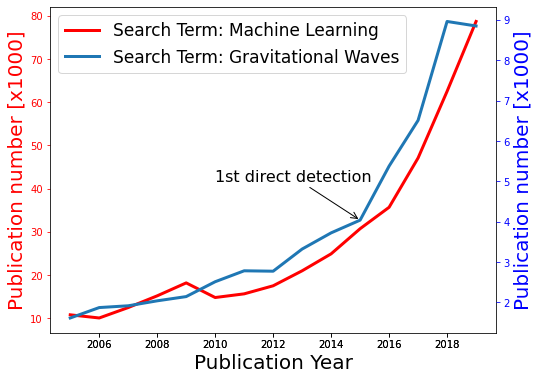
\includegraphics[width=.5\linewidth]{shared_resources/shared_figs/wos.png}
    \caption{Courtesy of WoS, nie lengthy caption WITH punctuation, make sure axes texts are large enough.}
    \label{fig:wos}
\end{figure}

\subsection{What are grav waves and how to detect - focus on transients (not spec BBH yet)}

*include key GW/GR equation(s)*

As hypothesised in GR (insert citation - the same one as abbot2016 obs) gravitational waves are stretching/deformation of space-time from spinning massive objects. sources can be spilt into two types: continous grav waves (CWs) and transient grav wave signals (GWs). Types of Cws are SN and...(2 citations at least) and much work has been done on these however in this work we are focussed on the latter transient signals which are formed of (something) and CBCs.

HOW THE DETECTORS WORK....link to detector improvements in next subsection....
Will talk here about michelson intereormeters and how the mirrors are used as test masses. Info on how sensitivity has been practically improved with each generational upgrade to the LSC observatories.

\begin{figure}[t!]
    \centering
    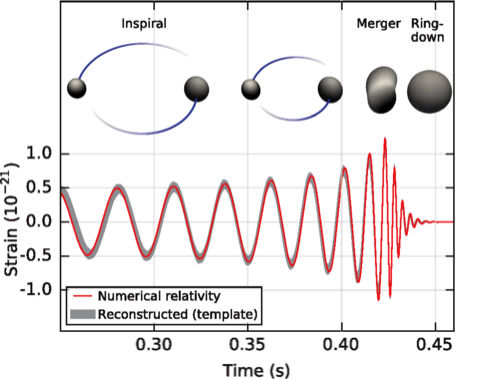
\includegraphics[width=.5\linewidth]{shared_resources/shared_figs/inspiral.png}
    \caption{Get good lengthy caption from abbot2016 observation paper.~\cite{abbott2016observation}}
    \label{fig:inspiral}
\end{figure}

\subsection{More info on detection pipelines - intro problems/ improvements for Bayesian and ML}

Here is where I will have a quick rundown of the 2 search-pipelines PyCBC~\cite{pycbc2016} and GstLal (gen1 - \cite{gstlal_gen1_2017}, gen2 - \cite{gstlal_gen2_2019})


Having completed both o3 runs the detectors are currently undergoing improvements in prep for o4 run with more detectors added (mention more detectors being added). Previous improvements between 02 and 03 runs are BLANK [citation to direct improvements paper - there are loads - maybe cite 2-3 here)] focusing on ASD (see figure~\ref{fig:asd})

Things we want to improve:
\begin{itemize}
    \item speed (multi-messenger)
    \item sensitivity (higher bandwidth)
    \item computational cost (allow for higher data rate)
    \item 
    
\end{itemize}



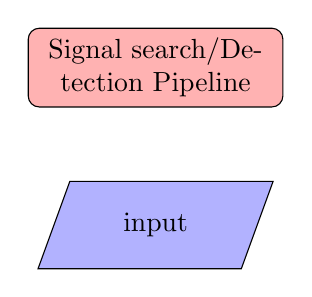
\begin{tikzpicture}[node distance=2cm][t!]

\node (start) [startstop] {Signal search/Detection Pipeline};
\node (label) [io, below of=start] {input};
\end{tikzpicture}

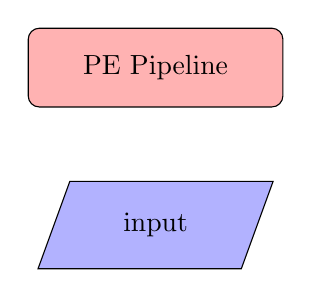
\begin{tikzpicture}[node distance=2cm][t!]

\node (start) [startstop] {PE Pipeline};
\node (label) [io, below of=start] {input};
\end{tikzpicture}

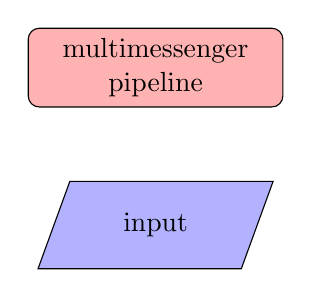
\begin{tikzpicture}[node distance=2cm][t!]

\node (start) [startstop] {multimessenger pipeline};
\node (label) [io, below of=start] {input};
\end{tikzpicture}






\section{Bayesian Inference ( (usefulness in pipeline)}

\subsection{intro of general bayesian stats with key equations}

\subsection{PE pipeline (Bayesian non-ML approach (old school))}
NOTE - Bayesian itself is a general method of stats/prob whereas *Bayesian Inference* is the direct data analysis method of getting posterior prob from prior and likelihood.

The below equations come from \cite{sivia2006textbook} and the og idea of bayes comes from the 18th centuerary paper post-humously publsihed \cite{bayesog}

\begin{equation}
\label{eq:bayes_equal}
P(\theta|\textbf{d}) = P(\theta ) \frac{P(\textbf{d} |\theta)}{P(\textbf{d})}
\end{equation}

\begin{equation}
\label{eq:bayes_propto}
P(\theta|\textbf{d}) \propto P(\theta ){P(\textbf{d} |\theta)}
\end{equation}

\section{Introductory machines learning}

\subsection{ML for GW - THEN specifically PE for CBC}

% \begin{itemize}
%     \item 
% \end{itemize}


\subsection{Variational Inference, specifics of CVAE and VItaminb and how it works and improvements we want to make}

\subsection{Home in on a specific improvement/new feature - Importance sampling (my practical project goal)}


\section{Plan for final report intro combine this with the preamble}

I have kept this literature review very general as, by virtue of such a complex topic that is new to me, and the cutting-edge nature of the research the exact nature of my project direction is being modified weekly. For my actual, needs to be ~7 pages (two col so more words but do want to start quite general but quickly get down to vit nitty gritty with specific NNs of vit and importance/rejection sampling: my knowledge in these topics isnt enough to write up yet. Also, by nature of the very specific methods of PE,sampling, CVAE etc, I have found that I have not grasped all aspects quite yet, so cannot write about them. The main things I am looking to work on before a final draft of intro will be completed:
\begin{itemize}
  \item Variational inference (VI) methods (expecting a presentation within the IGR-data group week beginning , specifically Conditional Variational Autoencoders (CVAE)
  \item Publication of O3b catalog
  \item Better practical working knowledge of tensorflow~\cite{tensorflow}
  \item want 100refs in total including software refs
  \item want a nice visual diagram for pipeline and mayeb in red where deep-learning is an option/getting injected.
\end{itemize}


\begin{figure}[t!]
     \centering
     \begin{subfigure}[t]{0.47\linewidth}
         \centering
         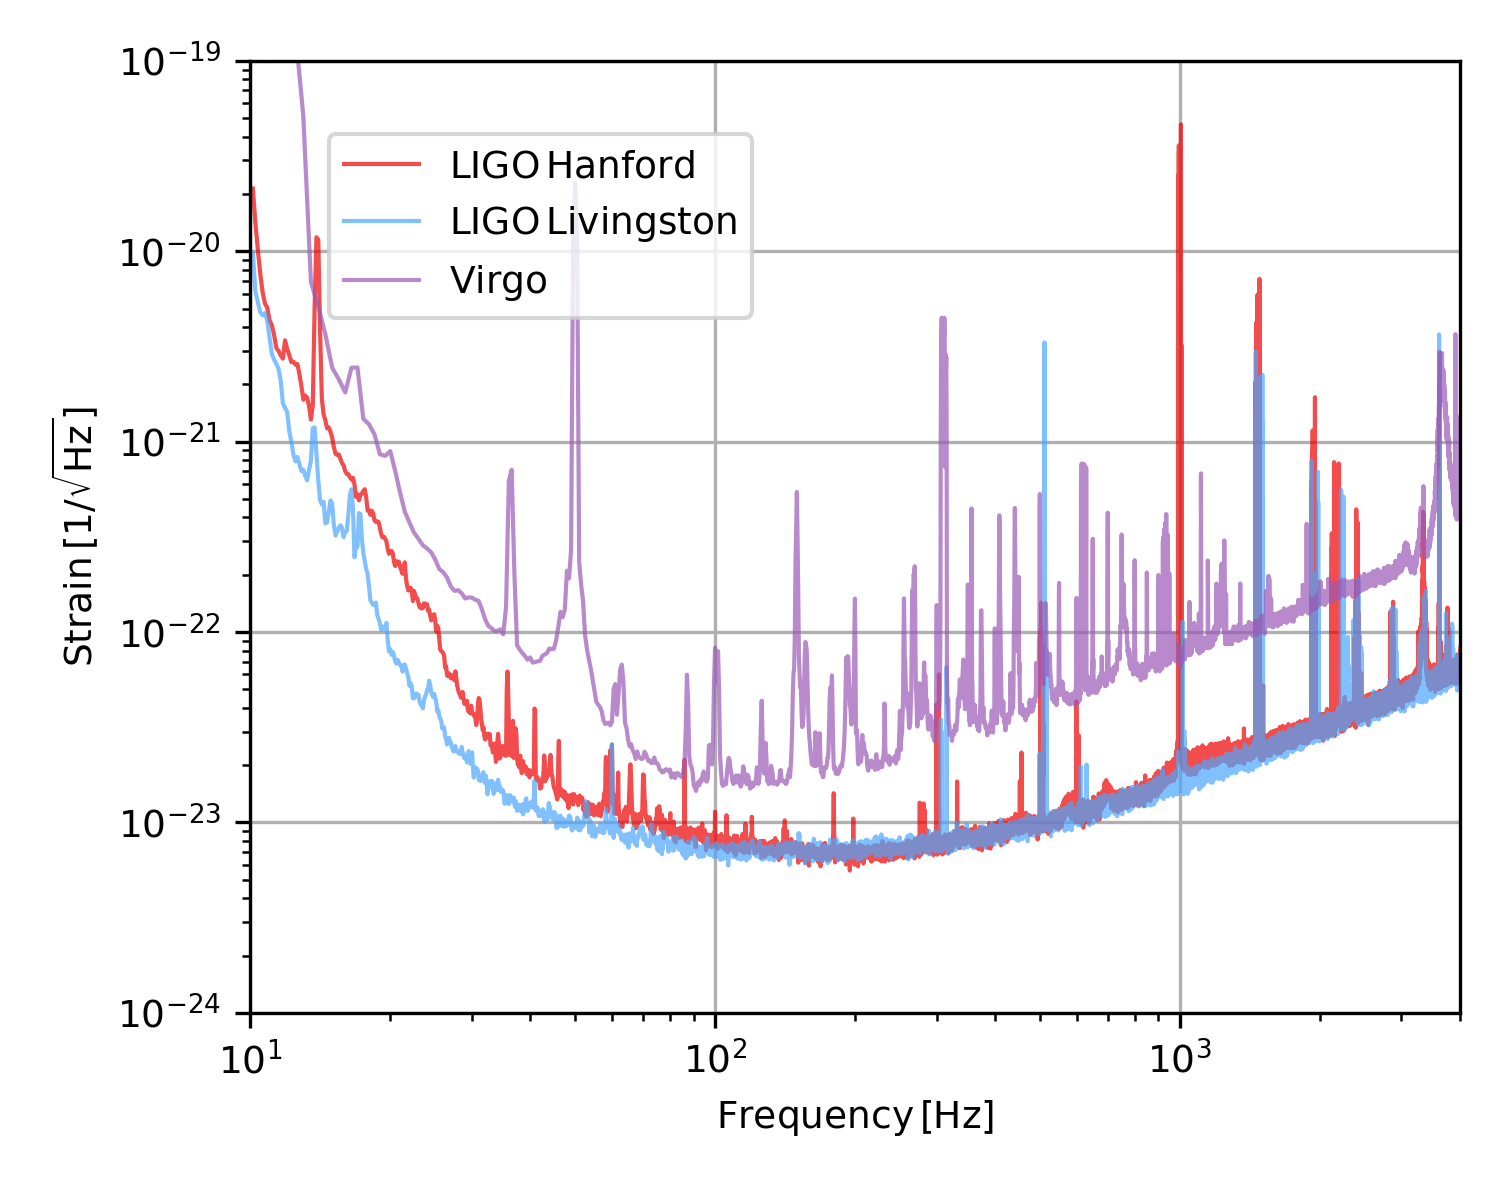
\includegraphics[width=\linewidth]{shared_resources/shared_figs/o2_asd.png}
     \end{subfigure}
     \begin{subfigure}[t]{0.47\linewidth}
         \centering
         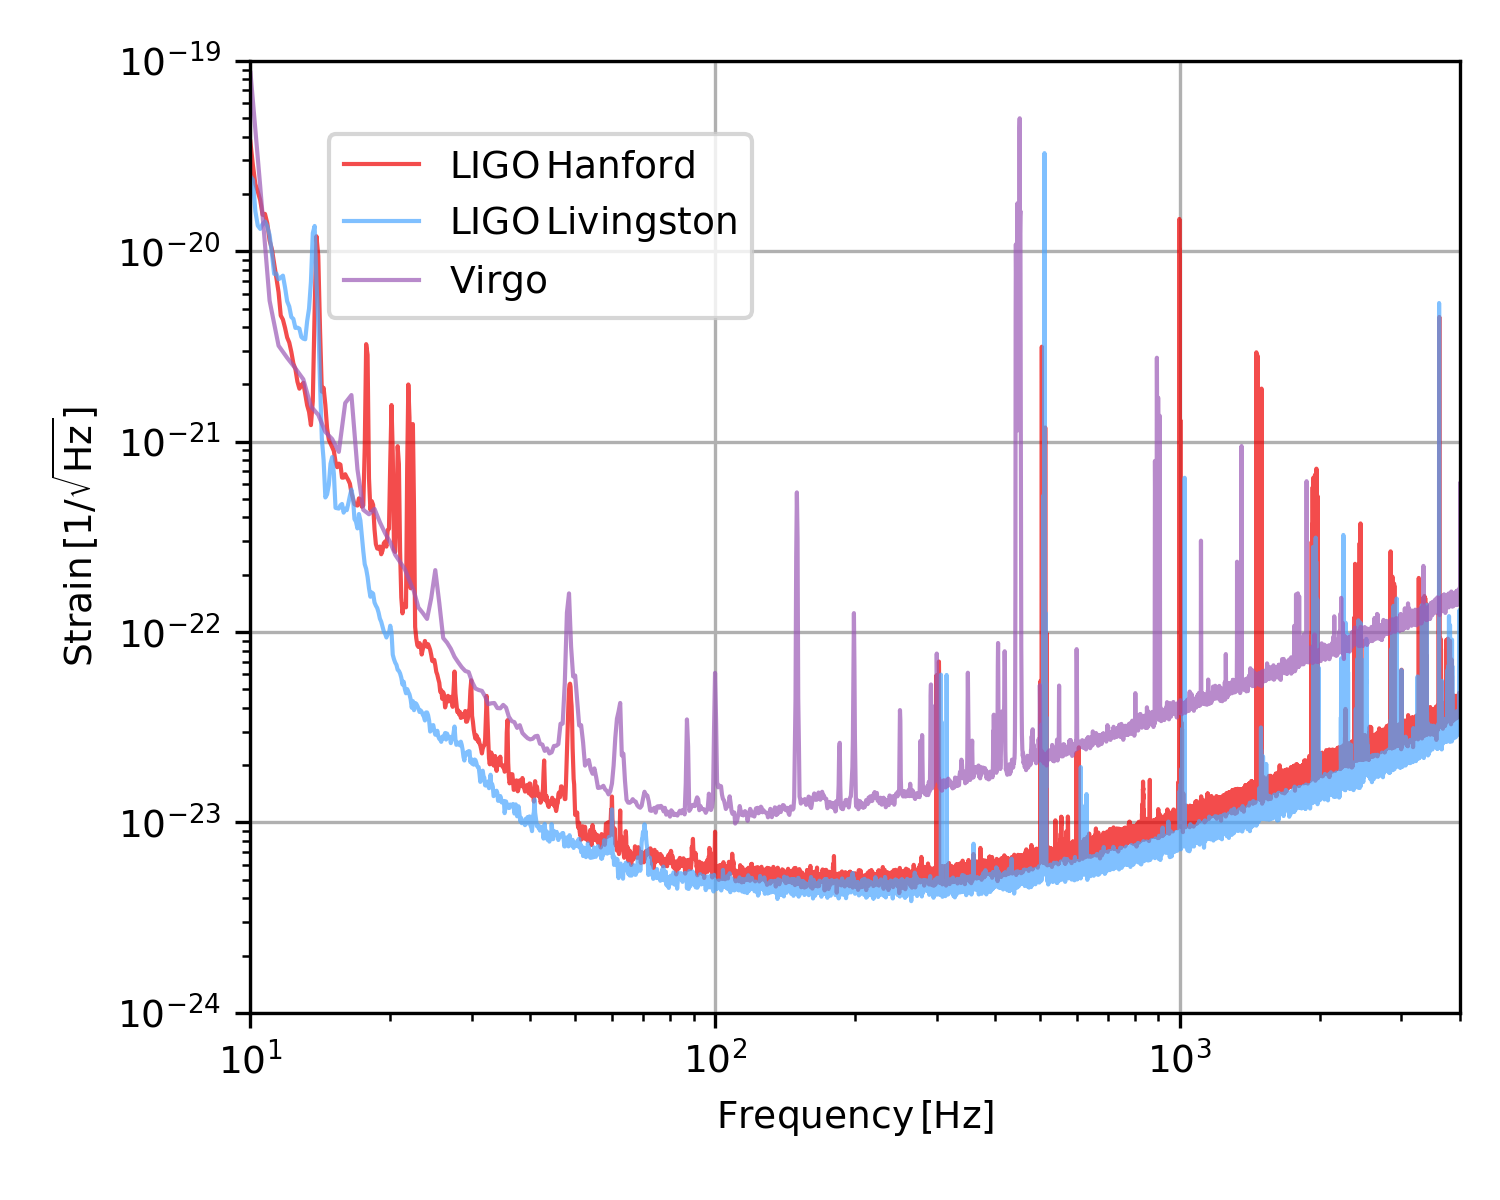
\includegraphics[width=\linewidth]{shared_resources/shared_figs/o3a_asd.png}
     \end{subfigure}
    %  \vspace*{-7mm}
     \caption{Raw data aquired and recreated inspired by \cite{gwtc1,gwtc2} ASD show better sensitivity for advanced LIGO between o2 and o3 (thanks to the improvements made - link to paper) VRIGO is also much improved - use Joes phd to talk about specific features of the ASD and how these have been improved between observations - then link to what improvementds are currently being made prepping for o4 run, Joes phd: \cite{bayley2020phd}} 
     \label{fig:asd}
\end{figure}

\begin{figure}[t!]
    \centering
    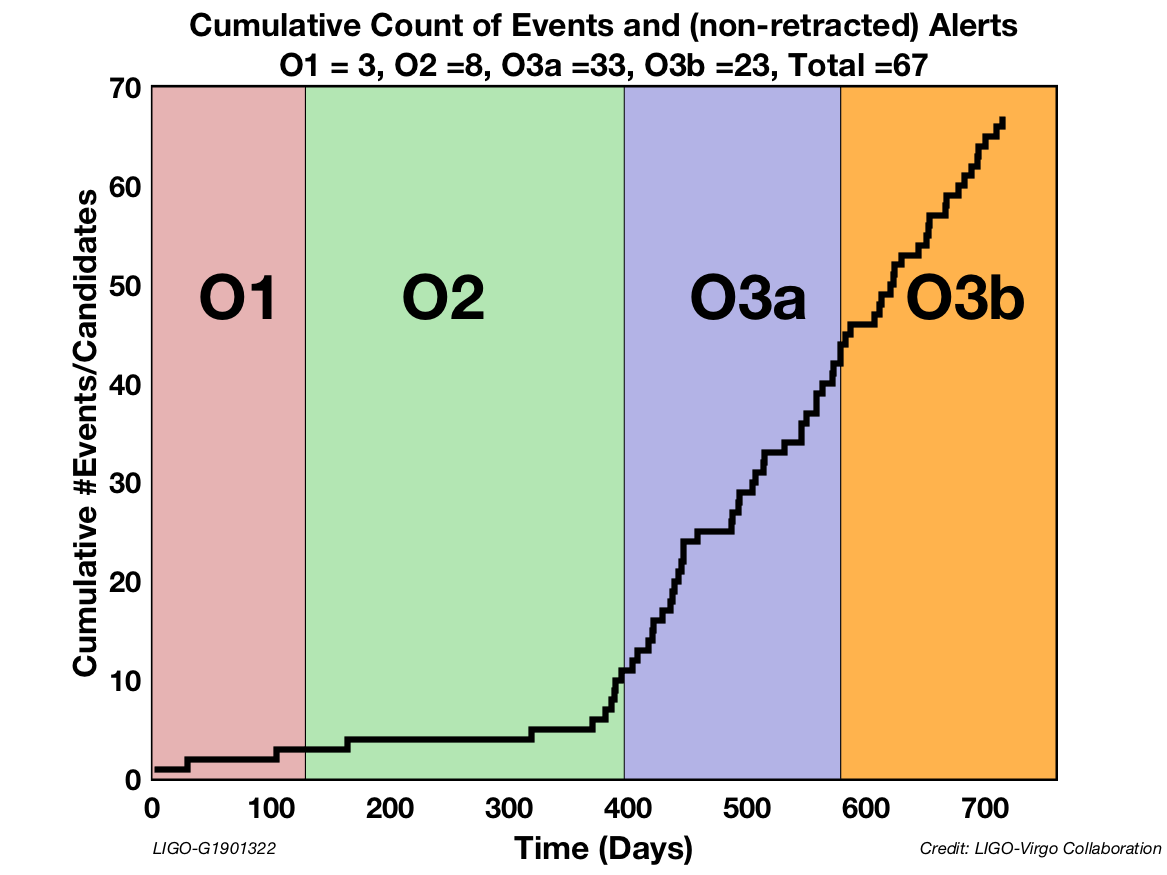
\includegraphics[width=.6\linewidth]{shared_resources/shared_figs/number_events.png}
    \caption{Adapted from data release document LIGO-G1901322-v25, as presented in fig 1 of Ref.~\cite{gwtc2}}
    \label{fig:events}
\end{figure}





\printbibliography



























































































\end{document}
